\documentclass{standalone}
\usepackage{tikz}
\usetikzlibrary{shapes.geometric}
\usepackage{ifthen}

\begin{document}

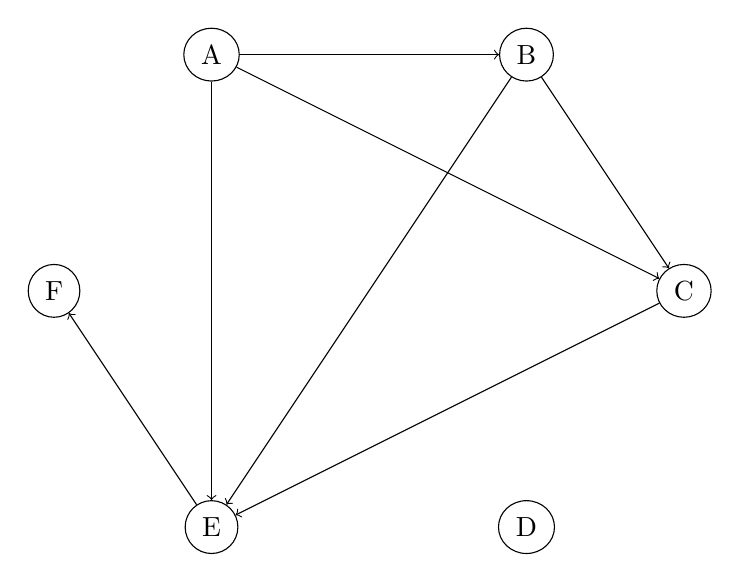
\begin{tikzpicture}
    \node[shape=ellipse,draw=black] (A) at (-2,5) {A};
    \node[shape=ellipse,draw=black] (B) at (2,5) {B};
    \node[shape=ellipse,draw=black] (C) at (4,2) {C};
    \node[shape=ellipse,draw=black] (D) at (2,-1) {D};
    \node[shape=ellipse,draw=black] (E) at (-2,-1) {E};
    \node[shape=ellipse,draw=black] (F) at (-4,2) {F};
    
    \path [->] (A) edge (B);
    \path [->] (A) edge (C);
    \path [->] (A) edge (E);
    \path [->] (B) edge (C);
    \path [->] (B) edge (E);
    \path [->] (C) edge (E);
    \path [->] (E) edge (F);
\end{tikzpicture}

\end{document}